% !TEX root = ../MemPod.tex
\section{Architecture}
\label{sec:Architecture}

Our clustered migration mechanism is designed to address key challenges associated with the migration problem. In this section, we first present a high-level overview of MemPod's proposed micro-architectural design, followed by a more detailed discussion regarding each building block. Throughout this section we also discuss some of the major design decisions of the state-of-the-art mechanisms.

%we present a complete description of our micro-architectural design, followed by a breakdown of the important design decisions, along with the corresponding challenge addressed by each one.


\begin{table*}[t]
  \ifOldResults
  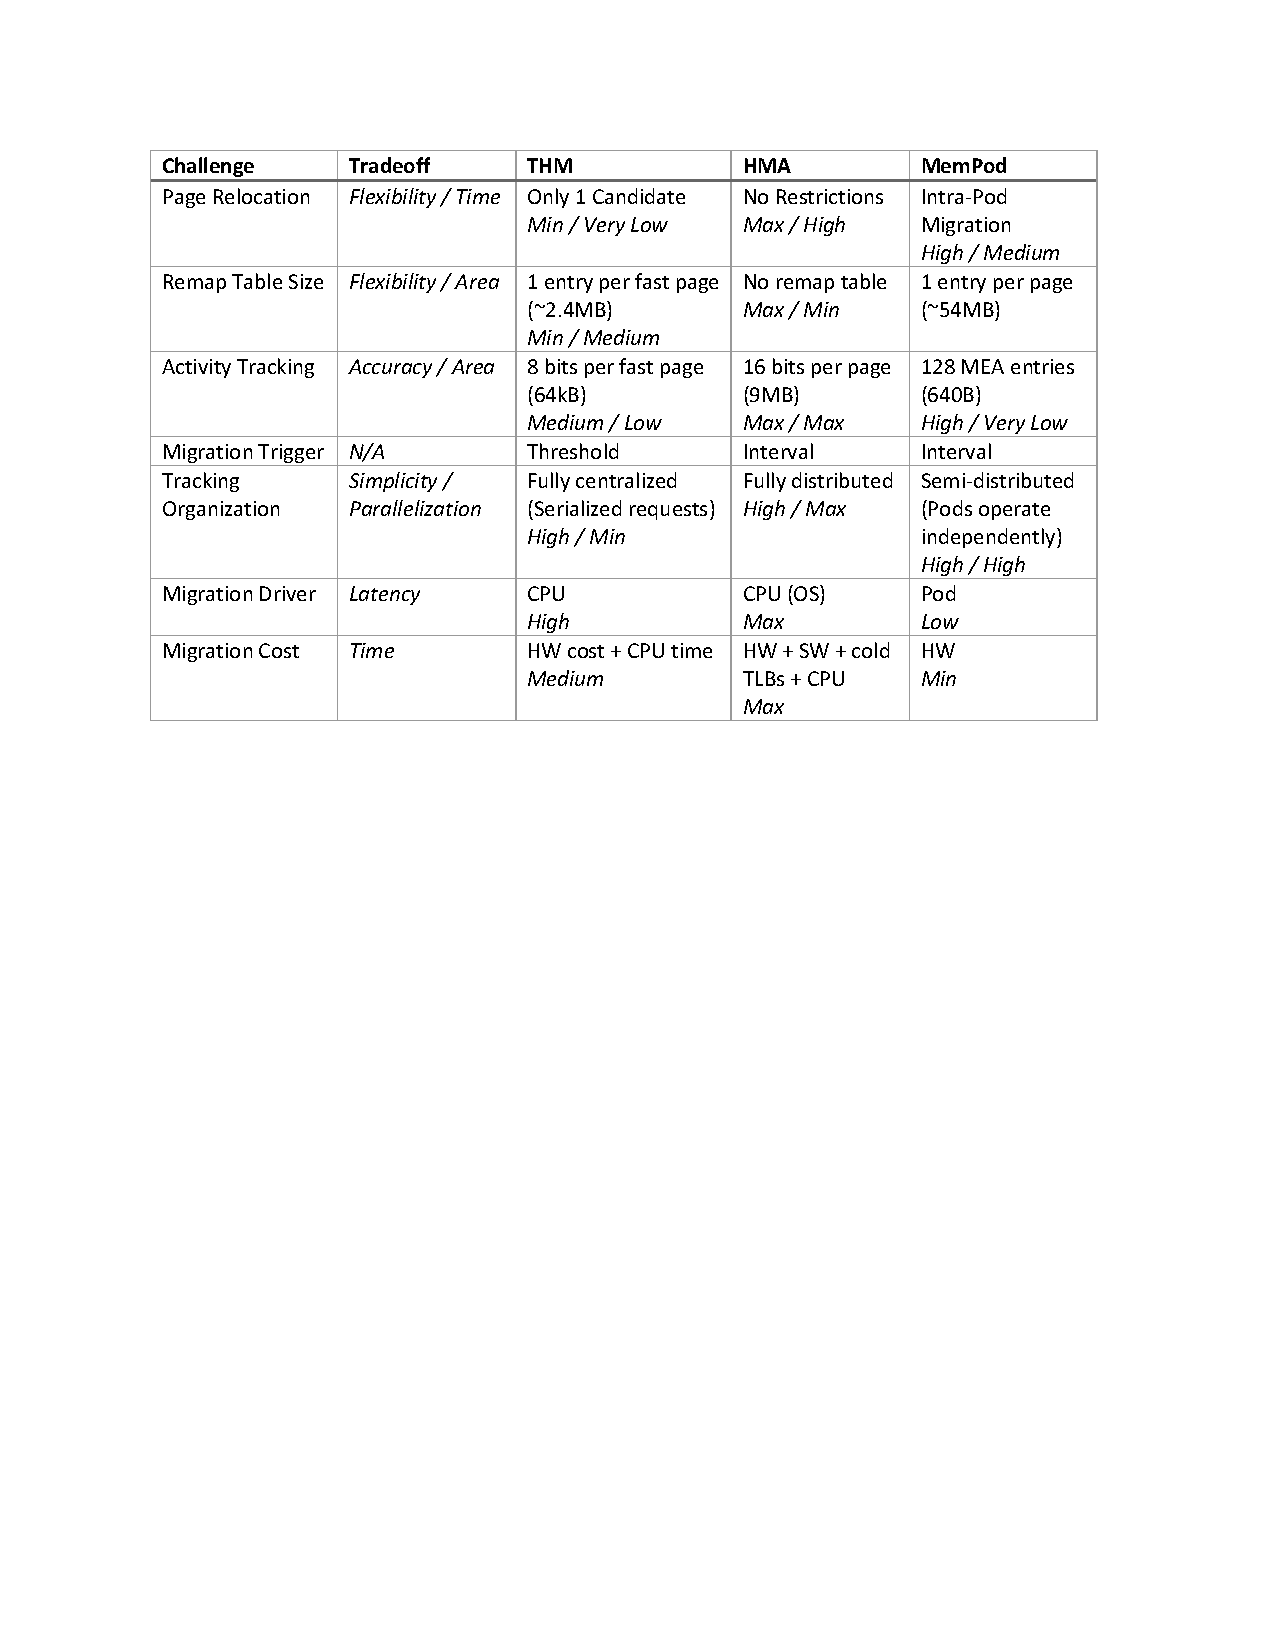
\includegraphics[width=\linewidth]{figures/comparison_table.pdf}
  \else
  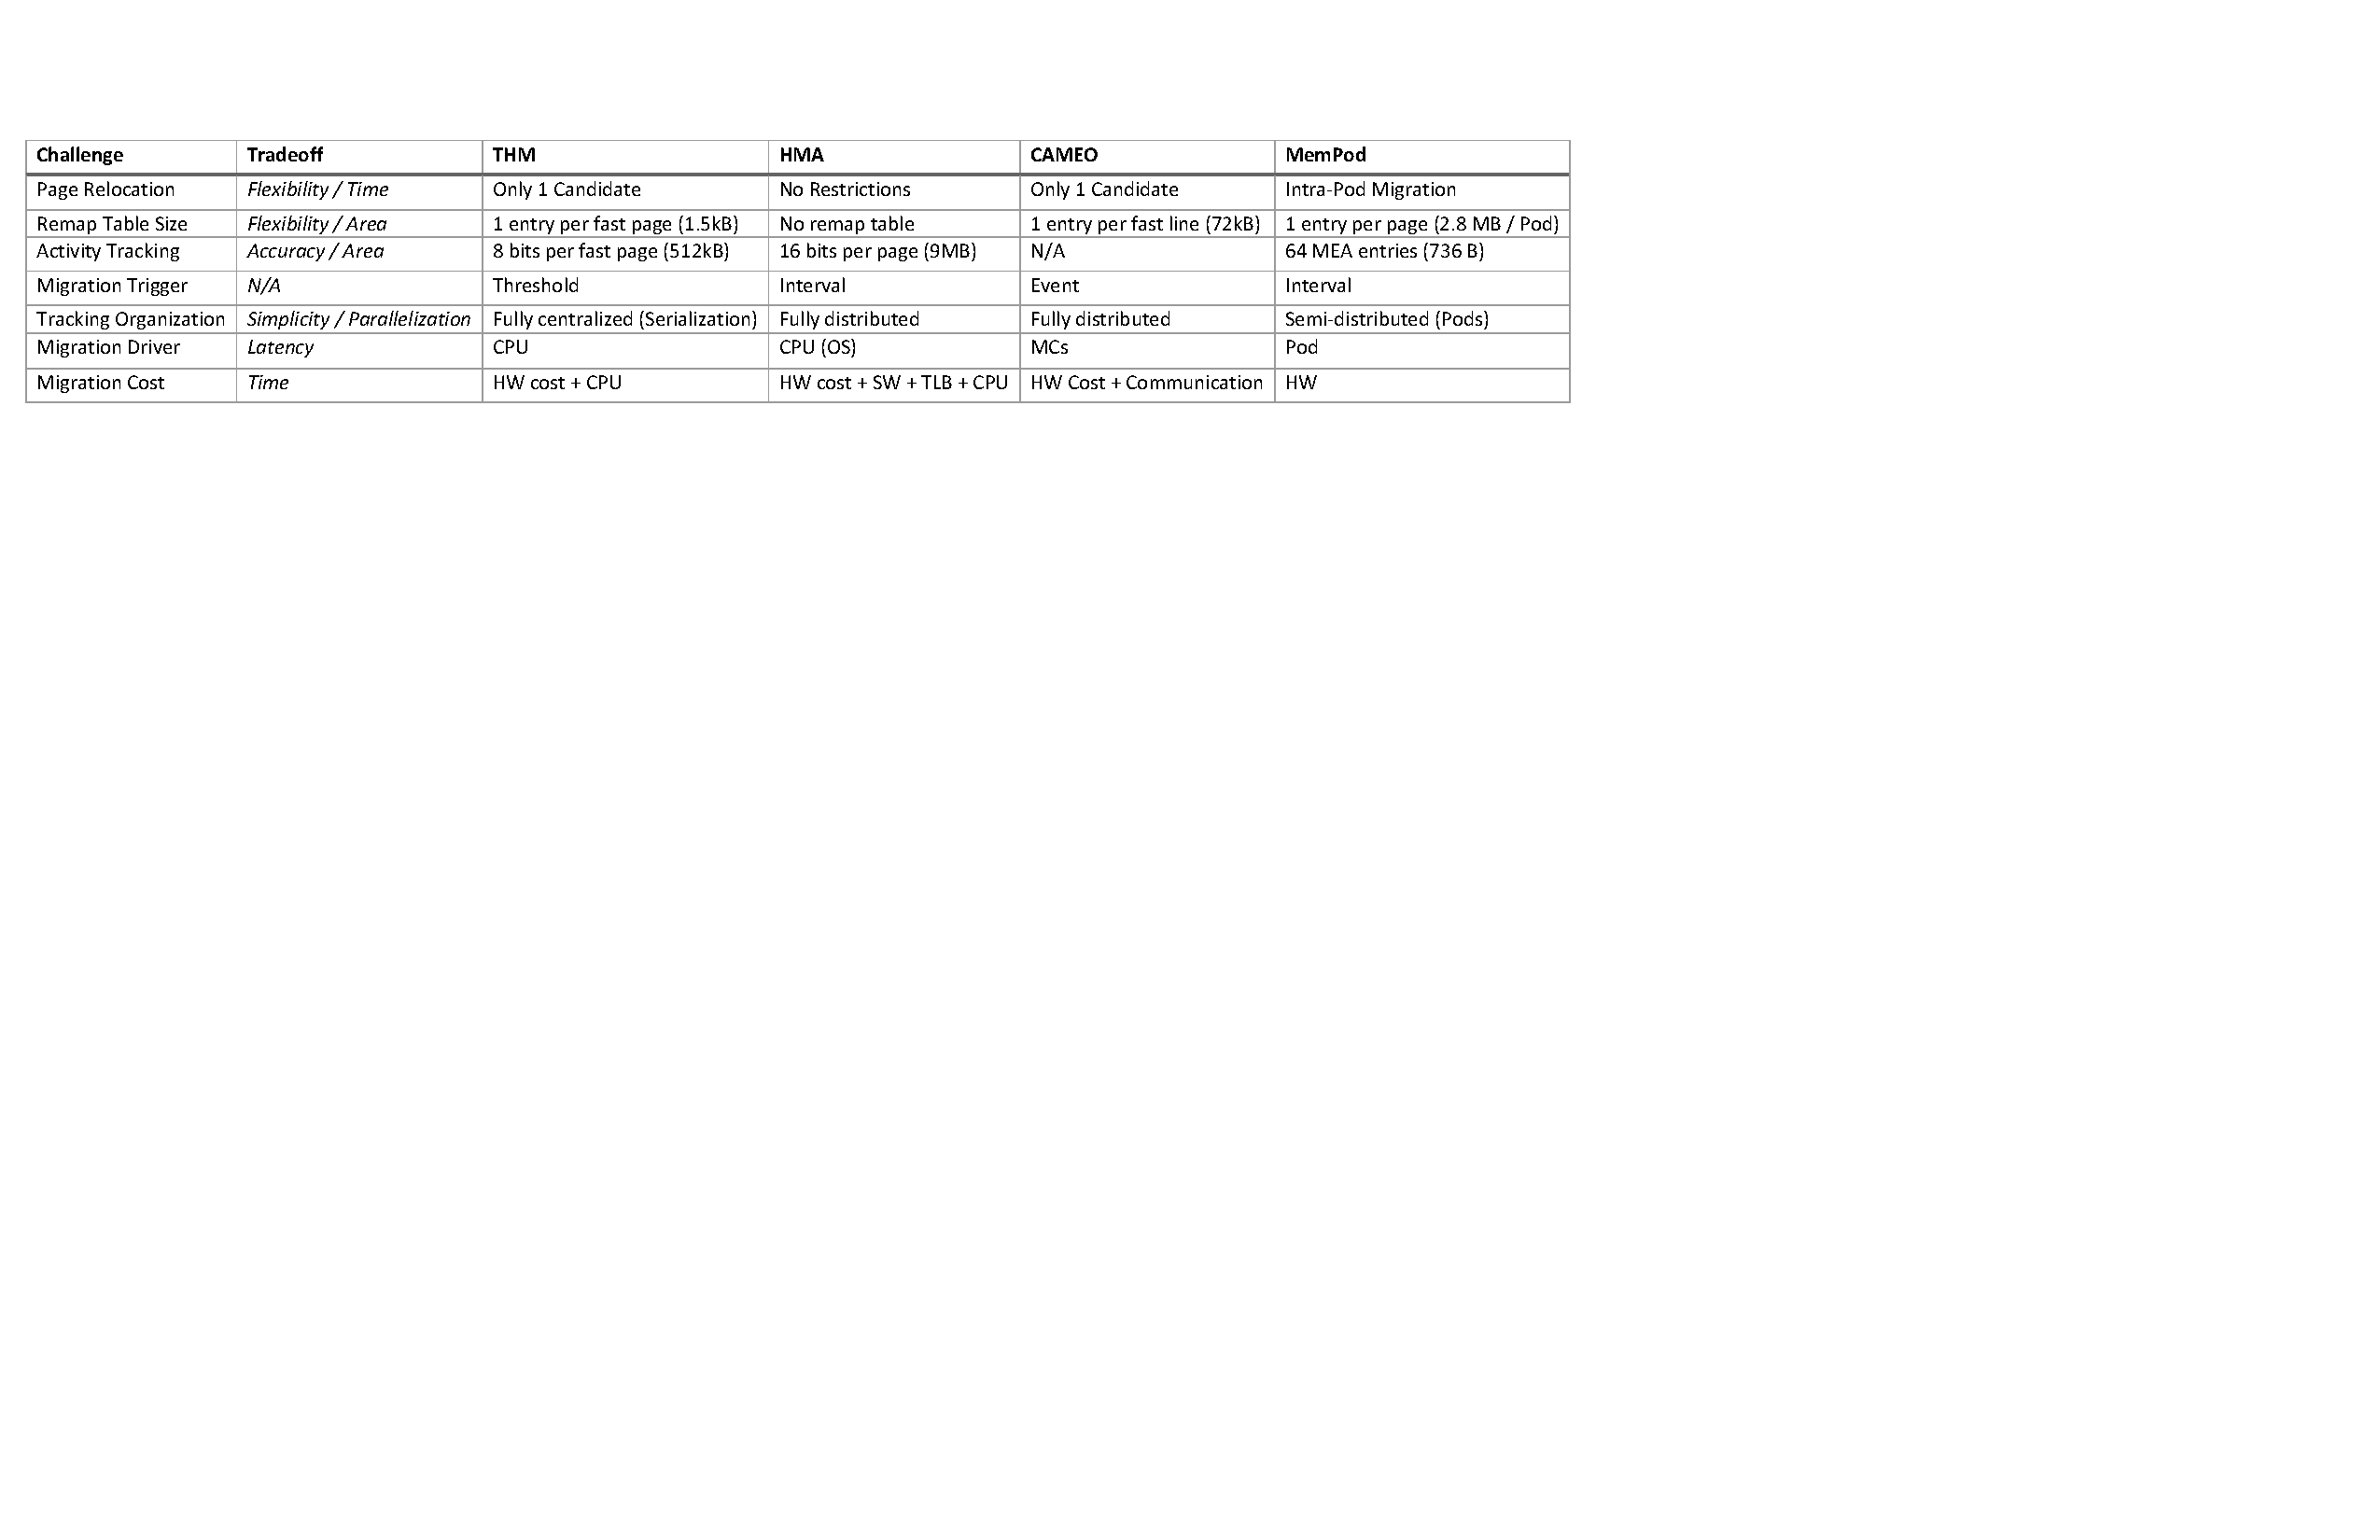
\includegraphics[width=\textwidth]{figures/revised/new/comparison_table.pdf}
  \fi
  \caption{Breakdown of state-of-the-art designs}
  \label{tbl:breakdown}
\end{table*}

\subsection{Clustered Migration Architecture}

 Figure \ref{fig:architecture_complete} presents an overview of MemPod. MemPod's design was kept modular to facilitate system integration and scalability. A number of memory ``Pods'' are injected between the Last Level Cache (LLC) and the system's memory controllers (MCs). Each Pod clusters a number of MCs and enforces migrations to only occur among its member MCs. Pods do not communicate with each other, preventing inter-Pod migrations. To the rest of the system, Pods are exposed as MCs. With MemPod's transparent design, each Pod will now be receiving all the requests originally addressed to any of the Pod's member MCs. 
 
\begin{figure}[h]
 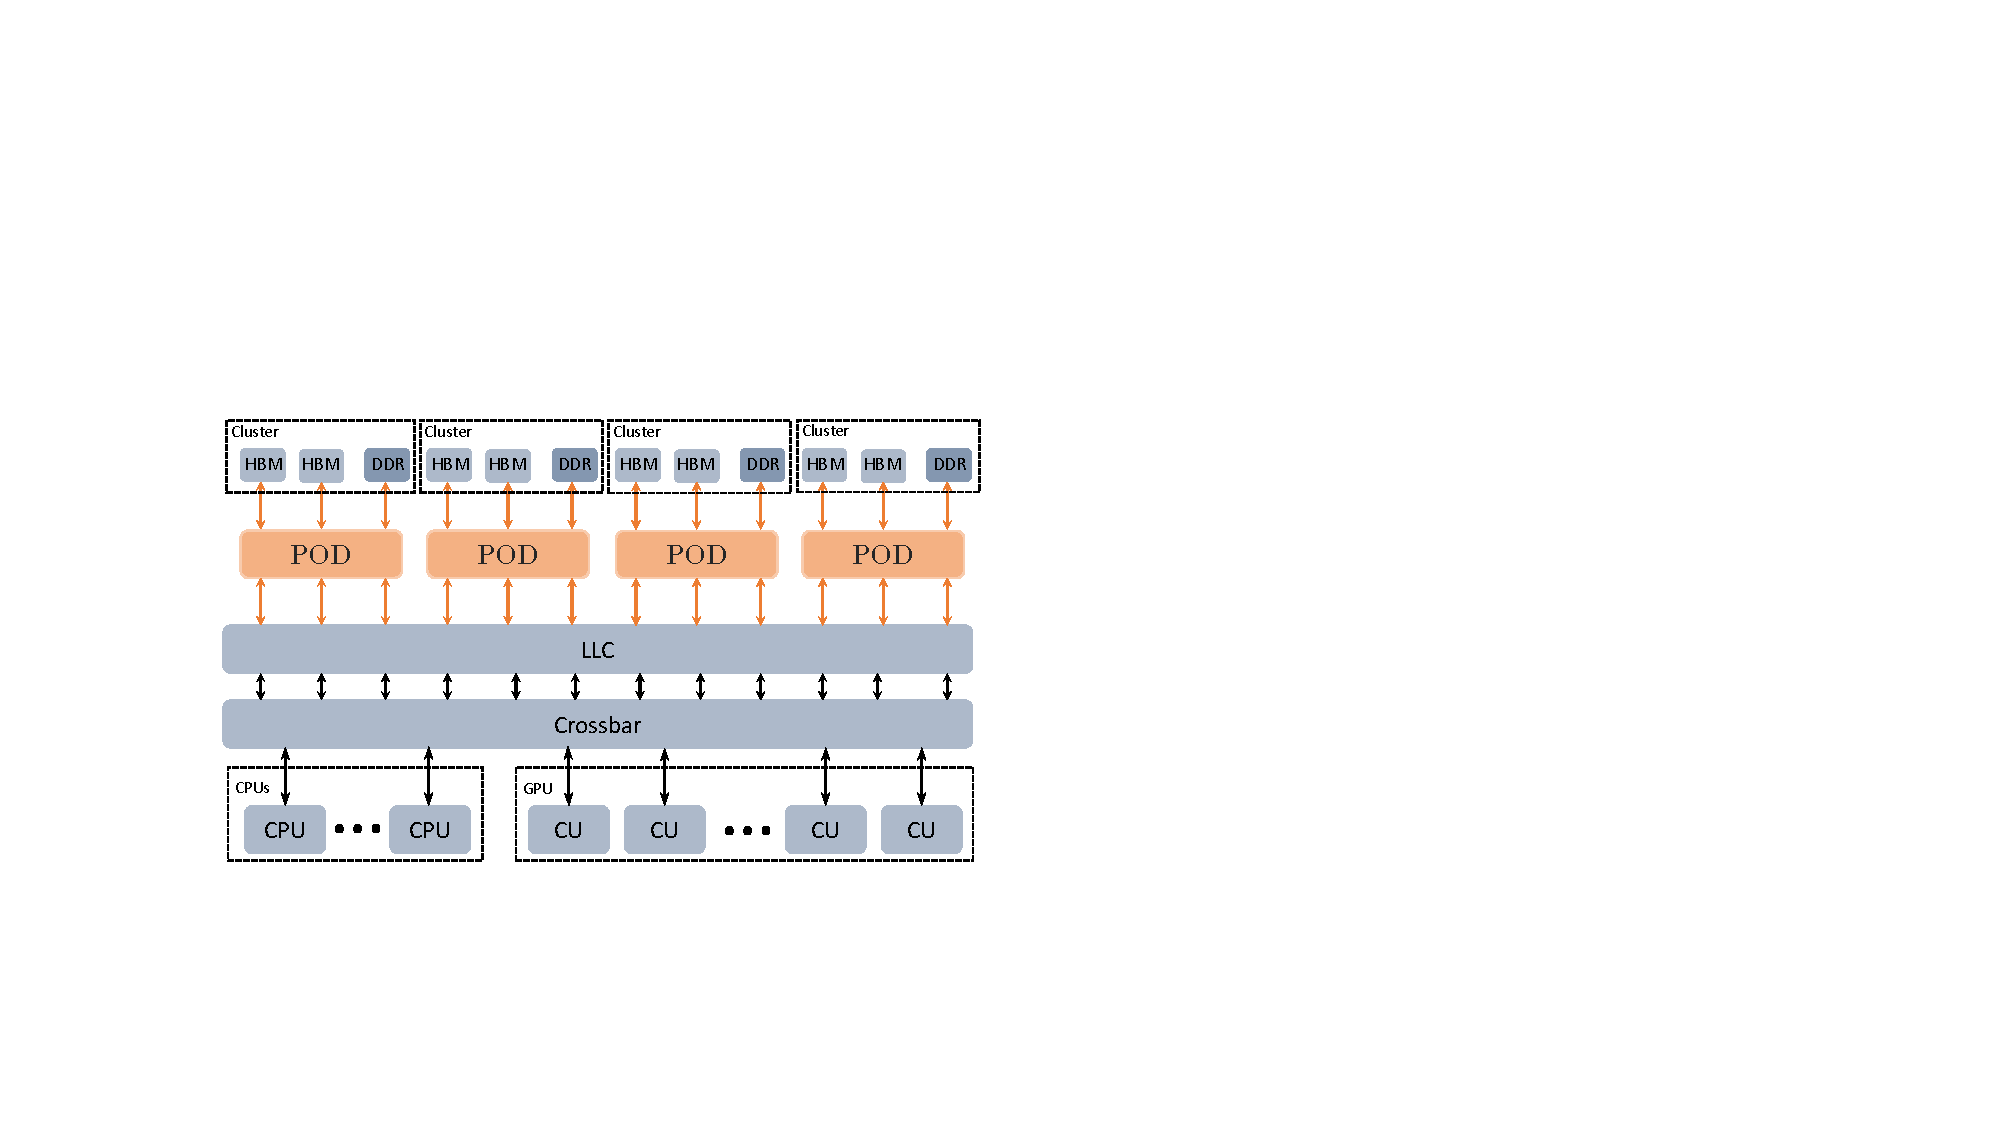
\includegraphics[width=0.47\textwidth]{figures/mempod_org.pdf}
 \caption{MemPod high-level architecture}
 \label{fig:architecture_complete}
\end{figure}

When a memory request arrives, the Pod monitors the request, updates any 
necessary migration-related activity tracking counters, and forwards 
the request to the intended recipient MC. The migration logic within a Pod does not need to be invoked during a response from any MC and can be bypassed to reduce memory access latency. A drawback of clustering MCs into Pods is the serialization of potentially parallel requests to different MCs of a single Pod. As such, activity tracking within a Pod as well as the subsequent forwarding of requests must be as efficient as possible. 

MemPod's clustered architecture also aids in reducing global traffic during migrations compared to non-partitioned mechanisms.  Because migration
traffic happens within a Pod, this architecture significantly reduces global
traffic and enables highly parallel migrations.
%  Higher global traffic could require the global switch (or crossbar) to have higher bandwidth resulting in increased energy costs and could also introduce performance penalties. Furthermore, with Pods servicing migrations transparently, the system's CPUs will be able to keep executing non-memory instructions during migrations. 

\subsubsection*{Memory Pod}

The major architectural elements of a Pod are shown in Figure \ref{fig:architecture_pod}. A Pod includes an activity tracking (MEA) unit, a remap table for keeping track of migrated pages and a forwarding unit that can re-encode a request with the relay address and, based on that address, send the request to the appropriate MC.
%
%\begin{figure}[h]
%  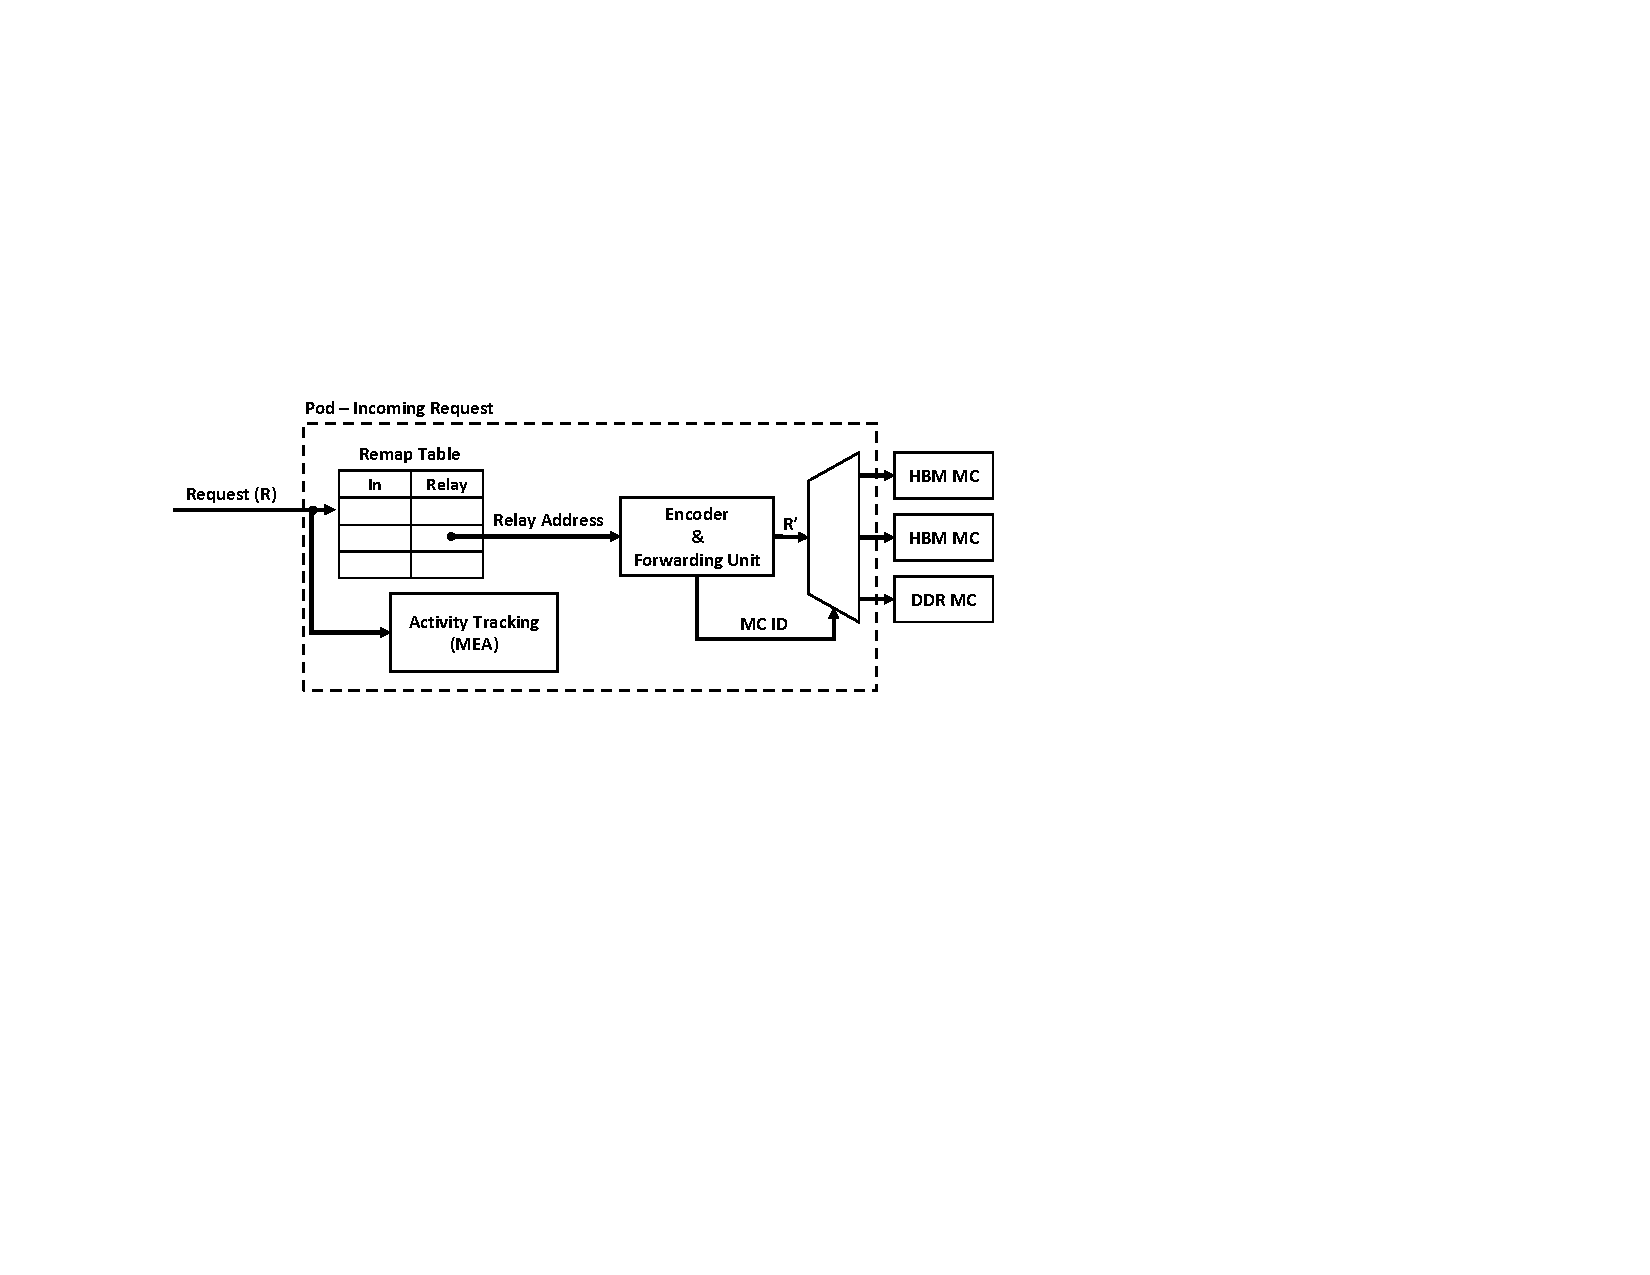
\includegraphics[width=0.46\textwidth]{figures/pod_design_request.pdf}
%  \caption{Major architectural Pod elements}
%  \label{fig:architecture_pod}
%\end{figure}

\begin{figure}
\begin{subfigure}{0.46\textwidth}
  \centering
  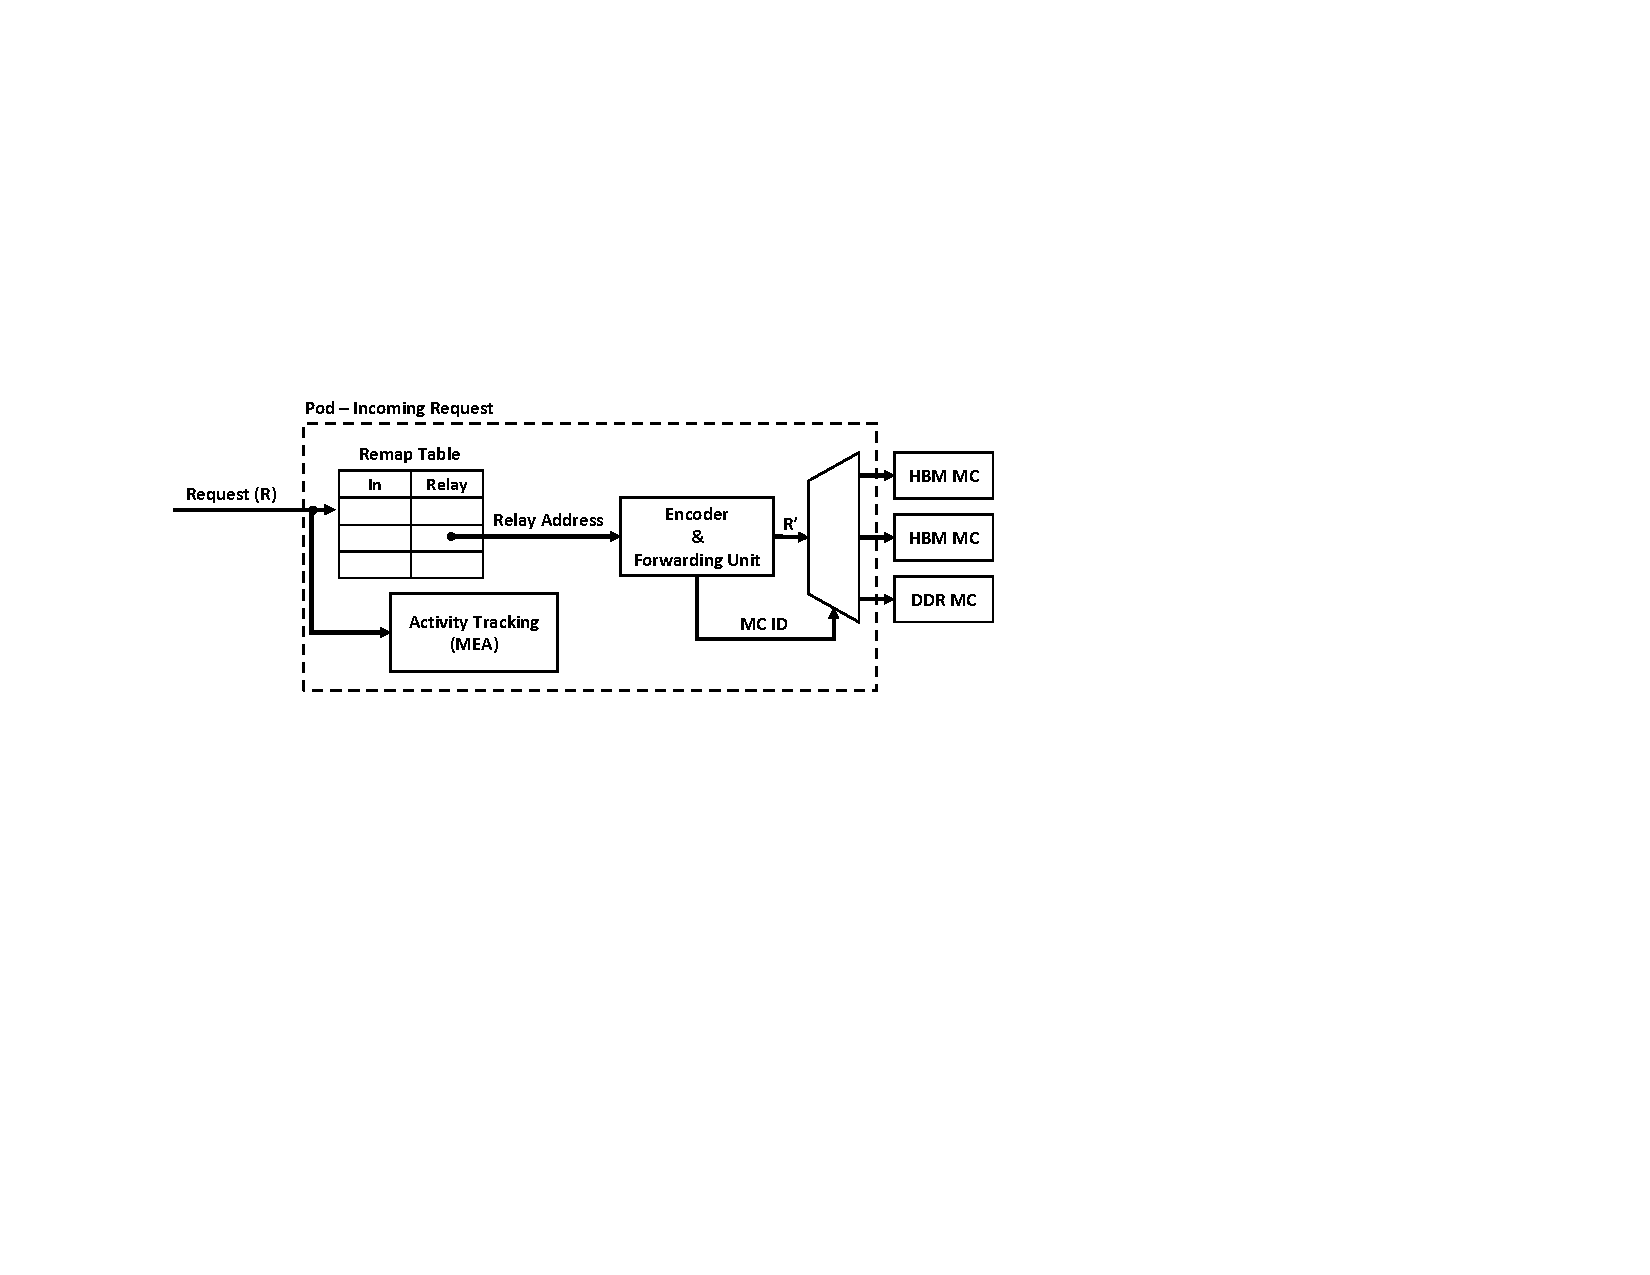
\includegraphics[width=\textwidth]{figures/pod_design_request.pdf}
  \caption{Pod's request forwarding operation}
\end{subfigure}%

\begin{subfigure}{0.46\textwidth}
  \centering
  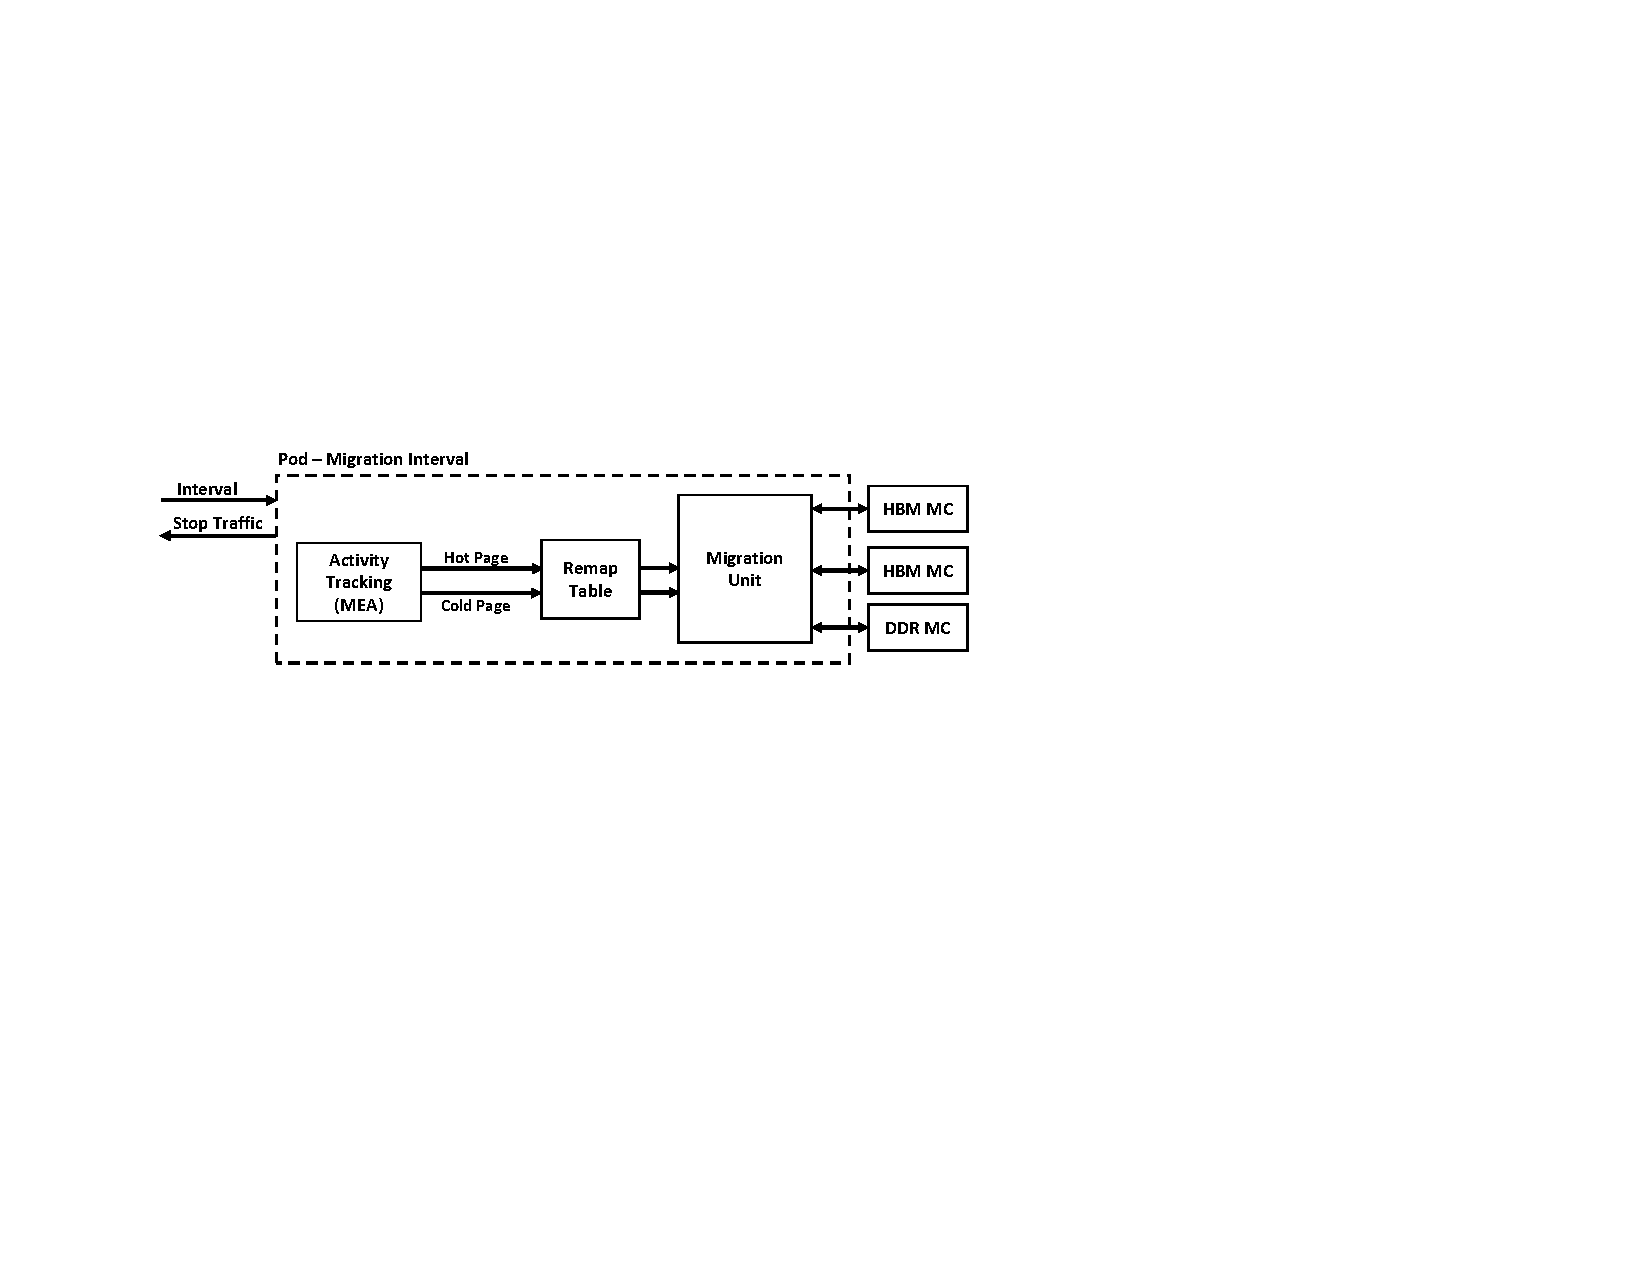
\includegraphics[width=\textwidth]{figures/pod_design_migration.pdf}
  \caption{Pod's migration procedure}
\end{subfigure}
\caption{Major architectural Pod elements}
\label{fig:architecture_pod}
\end{figure}

A designer can vary the parallelism and flexibility of MemPod by varying the
number of Pods. A design with one Pod is equivalent to a centralized 
migration controller allowing any-to-any migration,
while a design with a Pod number equal to the number of MCs would imply that migration is disabled. A reasonable design point would be to set the number of Pods equal to the number of slow-memory MCs. Such a configuration inherently restricts migration between slow off-chip channels, while at the same time maintaining full channel-level parallelism on the system's bottleneck: the slow MCs. In a configuration where the number of fast-memory MCs are not a multiple of slow-memory MCs, Pods can be configured asymmetrically or some MCs could be members of multiple Pods, with their capacity partitioned to avoid crosstalk issues. In Figure \ref{fig:architecture_complete} we present a system with eight MCs for the fast, on-die stacked memory and four MCs for the slow off-chip memory. Throughout this paper we use die-stacked HBM as the fast memory \cite{JEDEC-HBM-REVISED} and DDR4-1600 as our off-chip memory, and 
we set the number of Pods to four, as shown in Figure~\ref{fig:architecture_complete}.

\subsection{Building Blocks}

% Flexibility and Remap Table
MemPod imposes little migration restrictions since each slow page can migrate to any fast page location as long as it's within the same Pod. To support high flexibility MemPod requires a Remap Table structure capable of tracking all pages at each Pod and upon a lookup return the new address. The page table is updated to reflect changes with each migration. In addition to the remap table, our algorithm also needs to identify all pages currently mapped to fast memory (to identify a candidate to be evicted in favor of a new hot page). We do this with a smaller, inverted table that gives the original address of each page currently mapped to fast memory.

%Activity tracking
MemPod requires an MEA map structure of K entries, where K is the number of hot pages we wish to identify at each interval. Our evaluation presented in Section \ref{sec:Results} finds a good number of MEA counters to be 64. Each entry maps a page's address to a counter. Through our evaluation, we identified a good counter size to be 2 bits and 21 bits are needed to address each page within a Pod, leading to a total storage cost of 736B. Using the MEA counters, MemPod's activity tracking profiles \textit{every page in memory} with minimal hardware cost. 

% Migration Trigger
MemPod uses timing intervals. At each interval a Pod will migrate up to K pages into its fast memory, where K is the number of MEA counters used. MemPod is transparent to the system, rendering costly OS intervention unnecessary. Since each one of the N Pods will attempt to migrate up to K pages, up to N$\times$K migrations can happen within each interval. However, all Pods can perform their migrations in parallel. Due to MemPod's lightweight activity tracking, intervals can be kept very small, allowing each Pod to better adapt to the application's phase changes. Our evaluation shows a good interval length to be 50us.

% Migration Datapath
With the use of MEA counters, identifying the fast-memory page candidate is as simple as checking that it's not part of the K hot pages. The identification algorithm starts at the very first fast memory location and iterates sequentially until it detects a page address that is not in the set of hottest pages. For the next migration, the identification algorithm simply continues from where it was left. If a hot page already resides in the fast memory it is ignored.

In the state of the art mechanisms presented and evaluated in this paper, building block decisions vary significantly. HMA does not require a remap table due to the OS updating the existing system's structures. For activity tracking it uses Full Counters. The costly OS involvement and the high penalty for sorting all its counters force HMA to operate at very large intervals, weakening its adaptability to phase changes. However, HMA offers full flexibility for migrations.

THM offers significantly limited flexibility by restricting migrations withing segments, however this decision reduces bookkeeping costs significantly. Competing counters in each segment are used for activity tracking, occasionally leading to false (threshold-based) migration triggering if a cold page gets accessed at the right time. Identifying migration candidates incurs very little overhead since there is exactly one fast memory location for each slow memory page that triggers migration.

CAMEO operates similarly to THM, restricting migrations within segments (called congruence groups) but it operates at a finer granularity. Due to its finer granularity, it requires a larger remap table structure than THM. CAMEO does not require activity tracking since it uses an event based migration trigger performing a swap at each slow memory access. The process for identifying migration candidates is identical to THM's.

Table \ref{tbl:breakdown} shows a detailed comparison of all mechanisms' building block decisions, comparing their costs and presenting the tradeoff impact of each one.


\subsection{Distributed Migration Controllers}

\remark{A.P.: This used to be the Decentralization subsection. Let's see if it works better here. I'm basically rewriting the whole thing. The purpose of this subsection now is to explain the benefits of distributed migration controllers such as Pods compared to centralized units.}

Migration mechanisms in the literature \cite{sim-micro2014,cameo} assume a centralized migration controller which all memory requests have to go through before reaching the memory, in order to monitor memory activity, read remap tables and control migrations. MemPod's distributed migration controllers control every aspect of the migration process. The use of four Pods breaks the problem into smaller pieces in a divide-and-conquer approach. Instead of trying to identify the N best pages to migrate from the entire memory, each Pod now has to identify the $N\over4$ pages per Pod. Each Pod will also require lower bandwidth than a centralized unit as it handles a fraction of the traffic.

Prior publications \cite{loh-isca08} demonstrate that the layout and address interleaving of main memory and last level cache can be co-designed and benefit a system by increasing efficiency and reducing global traffic. The proposed designs align cache ``banks'' with main memory banks (among other optimizations). Even though not specifically proposed for 3D-stacked memories, if such a design is assumed, a centralized migration controller would be detrimental to the carefully designed alignment since all LLC misses will now have to go through the centralized unit and then fan back out to their respective MCs.

Finally, a clustered design ensures that we are never moving data across the entire system. Migration can only occur within a Pod and between ``sibling'' MCs. By limiting migration distance, MemPod imposes a tighter ceiling on data movement energy which can lead to migration-related energy savings when compared to a centralized design.
